\hypertarget{problem-6.8}{%
\section{Problem 6.8}\label{problem-6.8}}

\textbf{Problem statement:} Given a model of infectious disease spread
in a fixed population comprising either susceptible \emph{S} or infected
\emph{I} individuals, whose rates of change are represented as
\(dS/dt = -acSI + \sigma I\), and \(dI/dt = acSI - \sigma I\), where
\emph{a} is the probability of transmission, \emph{c} is the per-capita
contact rate between infected and susceptible individuals, and
\(\sigma\) is the recovery rate, we want to (a) prove that the
proportion of infected individuals \(P = I/(S+I)\) satisfies the
differential equation

\begin{equation} dP/dt = \alpha P(1 - P) - \sigma P \end{equation}

when \(\alpha = ac (S+I)\), (b) Determine the equilibria for \emph{P}
and their validity, (c) Determine the local stability of the equilibria
and its implications, (d) Sketch the shape of the differential equation
to determine the global stability of the equilibria, and (e) Determine
the the general solution of \emph{P}.

\hypertarget{a-proving-the-differential-equation-of-p}{%
\subsection{\texorpdfstring{(a) Proving the differential equation of
\emph{P}}{(a) Proving the differential equation of P}}\label{a-proving-the-differential-equation-of-p}}

Starting from equation (3), and substituting the value of \(P\):

\begin{equation} dP/dt = \frac{d\frac{I}{(S+I)}}{dt}  \end{equation}

Applying the quotient rule:

\begin{equation} dP/dt = \frac{dI}{dt} (I+S) - I \frac{d(I+S)}{dt} \end{equation}

and then expanding \(I d(I+S)/dt\):

\begin{equation} dP/dt = \frac{dI}{dt} (I+S) - I \frac{dI}{dt} - I \frac{dS}{dt} \end{equation}

and further cancelling oppositely signed \(I (dI/dt)\) leaves us the
following equation.

\begin{equation} dP/dt = S \frac{dI}{dt} - I \frac{dS}{dt} \end{equation}

Substituting the values of \(dI/dt\) and \(dS/dt\) as given:

\begin{equation} dP/dt = \frac{S(acSI - \sigma I) - I(-acSI + \sigma I)}{(I+S)^2} \end{equation}

and expanding:

\begin{equation} dP/dt = \frac{S^{2}acI - \sigma SI + acSI^2 - \sigma I^2}{(I+S)^2} \end{equation}

leaves us:

\begin{equation} dP/dt = \frac{ac(S+I) \cdot SI}{(I+S)^2} - \frac{\sigma I(I+S)}{(I+S)^2} \end{equation}

which, given \(\alpha = ac(S+I)\), and \(1 - P = S/(I+S)\), and on
converting all \(I/(S+I)\) to \(P\), satisfies the condition
\(dP/dt = \alpha P (1-P) - \sigma P\).

\hypertarget{b-equilibria-of-p}{%
\subsection{\texorpdfstring{(b) Equilibria of
\emph{P}}{(b) Equilibria of P}}\label{b-equilibria-of-p}}

One obvious equilibrium of \emph{P} is 0, since the infection does not
spontaneously arise. The upper equilibrium of \emph{P} can be found from
the osbervation that at equilibrium the rate of change of infection
status is 0, i.e., \(dP/dt = 0\). Hence at equilibrium:

\begin{equation} \alpha P (1-P) = \sigma P \end{equation}

and the second equilibrium value of \(P\),
\(\hat{P} = 1 - (\sigma/\alpha)\). Given that \emph{P} is a proportion,
\(\sigma/\alpha\) cannot be greeater than 1, or the rate of recovery
cannot be greater than the infectivity. In a special case of the
parameters, any starting \emph{P} is an equilibrium when infectivity and
recovery rates are equal.

\hypertarget{c-local-stability-of-equilibria}{%
\subsection{(c) Local stability of
equilibria}\label{c-local-stability-of-equilibria}}

Beginning with (3), the differential equation of \emph{P}, we
differentiate \(f(P)\) w.r.t. \(P\) so:

\begin{equation} \frac{df(P)}{dP} = \frac{d}{dP} \alpha P(1-P) - \sigma P \end{equation}

In \emph{Mathematica} the command
\texttt{D{[}\textbackslash{}Alpha\ P\ (1\ -\ P)\ -\ \textbackslash{}Sigma\ P,\ P{]}}
yields the derivative \(\alpha(1 - P) - \alpha P - \sigma\), which is
defined near the equilibria as:

\begin{equation} r \equiv df/dP|_{P = \hat{P}} = \alpha(1 - \hat{P}) - \alpha \hat{P} - \sigma \end{equation}

At each of the two equilibria, \(\hat{P} = 0\) and
\(\hat{P} = 1 - (\sigma/\alpha)\), the corresponding \(r\) is obtained
by substituting values of \(\hat{P}\): \(r_{0} = \alpha - \sigma\), and
\(r_{1 - (\sigma/\alpha)} = \sigma - \alpha\).

At \(\hat{P} = 0\), \(r\) is always positive since \(\sigma < \alpha\),
making it an unstable equilibrium, while \(r\) is always negative at
\(\hat{P} = 1 - (\sigma/\alpha)\), making it a stable equilibrium. There
are no oscillations in this one-variable, continuous-time model where
\(f(n)\) is not a function of time.

\hypertarget{d-global-stability-of-equilibria}{%
\subsection{(d) Global stability of
equilibria}\label{d-global-stability-of-equilibria}}

Assuming values of \(\alpha = 0.8\) and \(\sigma = 0.1\), the global
stability of (3) is shown in Figure 1 derived from \emph{Mathematica}
using:

\begin{lstlisting}[language=Mathematica]
f = \[Alpha] P (1 - P) - \[Sigma] P;

Plot[f /. \[Alpha] -> 0.8 /. \[Sigma] -> 0.1, {P, 0, 1},
 PlotTheme -> "Classic",
 PlotStyle -> {Black},
 AxesLabel -> {"P", "dP/dt"},
 PlotLabel -> "dP/dt ~ P, \[Alpha] = 0.8, \[Sigma] = 0.1"]

\end{lstlisting}

\begin{figure}
\centering
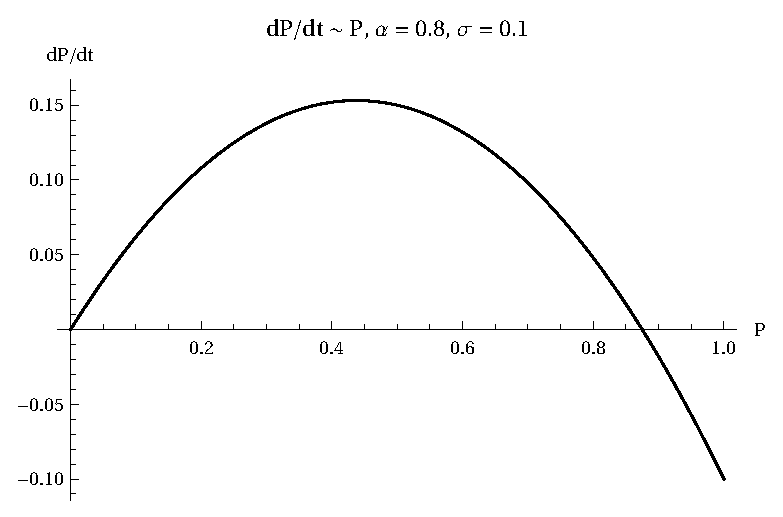
\includegraphics[width=0.5\textwidth,height=\textheight]{figChap6.8d.eps}
\caption{Differential equation dP/dt versus P, for values of \(\alpha\)
= 0.8, \(\sigma\) = 0.1. The equilibrium at P = 0 is unstable, while the
equilibrium at P = 0.875 is stable.}
\end{figure}

\hypertarget{e-general-solution-for-dpdt-alpha-p-1-p---sigma-p}{%
\subsection{\texorpdfstring{(e) General solution for
\(dP/dt = \alpha P (1-P) - \sigma P\)}{(e) General solution for dP/dt = \textbackslash{}alpha P (1-P) - \textbackslash{}sigma P}}\label{e-general-solution-for-dpdt-alpha-p-1-p---sigma-p}}

The general solution can be found with a separation of variables, where
\(f(P) = \alpha P (1-P) - \sigma P\), and \(g(t) = 1\). The itnegrals
for evaluation are

\begin{equation} \int \frac{1}{f(P)} dP = \int \frac{1}{\alpha P (1-P) - \sigma} dP \end{equation}

and \(\int g(t)dt = \int 1 dt = t + c\). The first integral (14) is
solved by passing it to \emph{Mathematica} using

\begin{lstlisting}[language=Mathematica]
iP = Integrate[1/(\[Alpha] P (1 - P) - \[Sigma] P), P];

FullSimplify[iP]

\end{lstlisting}

which yields

\begin{equation} \frac{ln(P) - ln[(P - 1)(\alpha + \sigma)]}{\alpha - \sigma} \end{equation}

This is equated to \(t + c\), and the whole equation solved for \(P(t)\)
using \emph{Mathematica}:

\begin{lstlisting}[language=Mathematica]
eq2 = iP == t + c;

FullSimplify[Solve[eq2, P]]

\end{lstlisting}

which gives the general solution

\begin{equation} P(t) = \frac{e^{(c+t)\alpha} (\alpha - \sigma)}{\alpha e^{(c+t) \alpha} - e^{(c+t) \sigma}} \end{equation}

\begin{center}\rule{0.5\linewidth}{\linethickness}\end{center}
